\documentclass[a4paper,twocolumn,10pt]{article}
\usepackage[spanish]{babel}
\usepackage[T1]{fontenc}
\usepackage[utf8]{inputenc}
\spanishdecimal{.}
\usepackage{lmodern}
\usepackage[a4paper]{geometry}
\usepackage{graphicx}
\usepackage{flushend}
\usepackage{wallpaper}
\usepackage{amsmath}
\usepackage{float}
\usepackage{colortbl}
\usepackage[normalem]{ulem}
\useunder{\uline}{\ul}{}
\usepackage[
backend=biber,
style=phys,
sorting=ynt
]{biblatex}
\addbibresource{biblio.bib}
\usepackage{csquotes}

\newcommand{\braket}[1]{ \langle #1 \rangle }

\begin{document}

\title{Experimento de Franck-Hertz}
\author{ \\Aldo Aliaga, Benjamín Yapur, Fabian Trigo \\ \textit{Departamento de Física y Astronomía, Universidad de Valparaíso}}
\twocolumn[
  \begin{@twocolumnfalse}
    \maketitle
    \begin{abstract}
  
    \end{abstract}
  \end{@twocolumnfalse}\bigskip]

\vspace{2cm}

\section{Introducción}
En este experimento lo principal son los electrones y átomos de Mercurio en el experimento original, en el presente se reemplazó por Argón
\subsection{Colisiones inelasticas}
En las colisiones elasticas, el electron impacta contra el atomo y continua con la misma velocidad antes del impacto pero con direccion distinta, cuando las velocidades son elevadas (sobre $1.3 M [m/s]$ las colisiones se vuelven inelasticas, de aqui en adelante en lugar de hablar de velocidades se hablará de energia, la cual en el caso listado corresponde a $4.9 [eV]$ para el atomo de Mercurio) entonces alli la velocidad del electron cambia, pues el atomo de Mercurio absorbe energia y la reemite en forma de radiacion.

Esta radiacion corresponde de acuerdo a la teoria de Bohr \cite{bohr} de la cuantizacion de niveles de energia; el atomo de Mercurio/Argón al abosrber energia del electron (absorber energia de su velocidad) sus electrones internos suben de un nivel de energia a otro, mediante la formula de Rydberg derivada en el articulo anterior \cite{rydberguv}:
\begin{equation}\label{eq:rydberg}
    \frac{1}{\lambda} = \frac{m_e Z^2 e^4}{8 h^3 c} (
    \frac{1}{n^2} - \frac{1}{m^2}    
    )
\end{equation}

donde $Z$ es la cantidad de protones en el nucleo, donde $m$ es el nivel externo y $n$ el nivel interno, esta formula se utiliza para la emisión de fotones con longitud de onda $\lambda$, para el presente experimento el Argón el salto del los dos primeros niveles adyacentes da una emision con longitud de onda: $\lambda = 108.1 [nm]$; utilizando la cuantizacion de energia de planck:
\begin{equation}\label{eq:planck}
    \Delta E = h \nu = h\frac{c}{\lambda}
\end{equation}


\section{Montaje Experimental}
\begin{figure}[H]
    \centering
    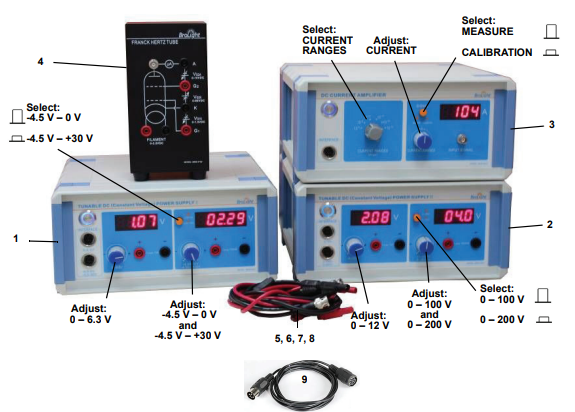
\includegraphics[width=0.4\textwidth]{Imagenes/FranckHertz/lista_exp.png}
    \caption{Lista de Elementos Experimento}
    \label{fig:listaelementos}
\end{figure}
\subsection{Herramientas}
\begin{itemize} 
\item Fuente de Poder I DC - Modelo SE-6615
\item Fuente de Poder II DC - Modelo SE-9644
\item Amplificador de Corriente DC - Modelo SE-6621
\item Tubo de Argon - Modelo SE-9650
\item Cables de conexion 
\item Cable BNC
\end{itemize}
Sigase el siguiente esquema de circuito, teniendo en cuenta los limites de voltaje especificados por el tubo de argón
\begin{figure}[H]
    \centering
    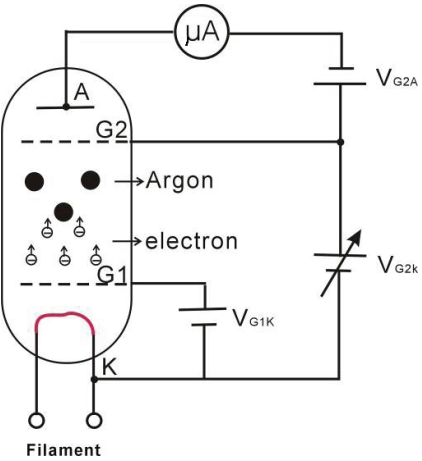
\includegraphics[width=0.4\textwidth]{Imagenes/FranckHertz/circuit.png}
    \caption{Circuito Tubo de Argón}
    \label{fig:argoncircuiot}
\end{figure}
ha de alimentarse con una diferencia de potencial el filamento $V_H$, junto a este filamento se tiene un punto de referencia K el cual esta cargado negativamente; la grilla G1 se encarga de acelerar los electrones, entre G1 y K existe una diferencia de potencial $V_{G1K}$ de manera que los electrones van desde K hacia G1 acelerando (con energia cinetica). 

Luego los electrones entre G1 y G2 (grilla 2) poseen la diferencia de potencial principal la cual se encargó de entregarles la mayor parte de energia de manera que posean suficiente para colisionar con los atomos de Argón en colisiones inelasticas; tengase en cuenta que existe tambien una diferencia de potencial entre G2 y K $V_{G2K}$, por tanto comparte el cable del negatiov con G1.

Entonces antes de llegar al punto A donde son finalmente medidos, se dejó una diferencia de potencial que se opone a los electrones que entran $V_{G2A}$, cuando los electrones han perdido energia debido a las colisiones no tienen suficiente para sobrepasar esta diferencia de voltaje, permitiendo asi al experimentador filtrar aquellas colisiones y hacerlas visibles en el analisis.

\begin{figure}[H]
    \centering
    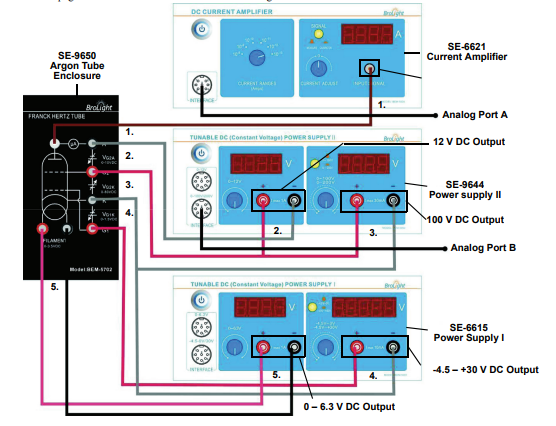
\includegraphics[width=0.4\textwidth]{Imagenes/FranckHertz/circuit_connections.png}
    \caption{Conexiones}
    \label{fig:conexiones}
\end{figure}

\section{Análisis}



\section{Conclusión}

\medskip

\printbibliography

\end{document}
 

